%%%% ijcai19.tex

\typeout{IJCAI-19 Instructions for Authors}

% These are the instructions for authors for IJCAI-19.

\documentclass{article}
\pdfpagewidth=8.5in
\pdfpageheight=11in
% The file ijcai19.sty is NOT the same than previous years'
\usepackage{ijcai19}

% Use the postscript times font!
\usepackage{times}
\usepackage{soul}
\usepackage{url}
\usepackage[hidelinks]{hyperref}
\usepackage[utf8]{inputenc}
\usepackage[small]{caption}
\usepackage{subfig}
\usepackage{graphicx}
\usepackage[none]{hyphenat}
\usepackage{amsmath}
\usepackage{booktabs}
\usepackage{algorithm}
\usepackage{algorithmic}
% \usepackage{epstopdf}
\usepackage{makecell}
\usepackage{float}
\usepackage{listings}
\urlstyle{same}

\usepackage{tikz}
\usetikzlibrary{calc, snakes}

% the following package is optional:
%\usepackage{latexsym}

% Following comment is from ijcai97-submit.tex:
% The preparation of these files was supported by Schlumberger Palo Alto
% Research, AT\&T Bell Laboratories, and Morgan Kaufmann Publishers.
% Shirley Jowell, of Morgan Kaufmann Publishers, and Peter F.
% Patel-Schneider, of AT\&T Bell Laboratories collaborated on their
% preparation.

% These instructions can be modified and used in other conferences as long
% as credit to the authors and supporting agencies is retained, this notice
% is not changed, and further modification or reuse is not restricted.
% Neither Shirley Jowell nor Peter F. Patel-Schneider can be listed as
% contacts for providing assistance without their prior permission.

% To use for other conferences, change references to files and the
% conference appropriate and use other authors, contacts, publishers, and
% organizations.
% Also change the deadline and address for returning papers and the length and
% page charge instructions.
% Put where the files are available in the appropriate places.

\title{Watercolor rendering and caustics effect for underwater scene} % TODO: TRANSLATE TO FRENCH MAYBE

% Multiple author syntax (remove the single-author syntax above and the \iffalse ... \fi here)
% Check the ijcai19-multiauthor.tex file for detailed instructions

\author{
Arnaud Paré-Vogt
\and
Mehdi Chaid
\affiliations
Département GIGL Polytechnique Montreal\\
\emails
arnaud.parevogt@gmail.com, % TODO: UPDATE WITH POLYMTL EMAIL
mehdi.chaid@polymtl.ca
}

\begin{document}
\lstset{language=C++}
\makeatletter
\g@addto@macro\@maketitle{
  \begin{figure}[H]
  \setlength{\linewidth}{\textwidth}
  \setlength{\hsize}{\textwidth}
  \centering
  \centering
  \subfloat[Scene with simple diffuse light.]{
      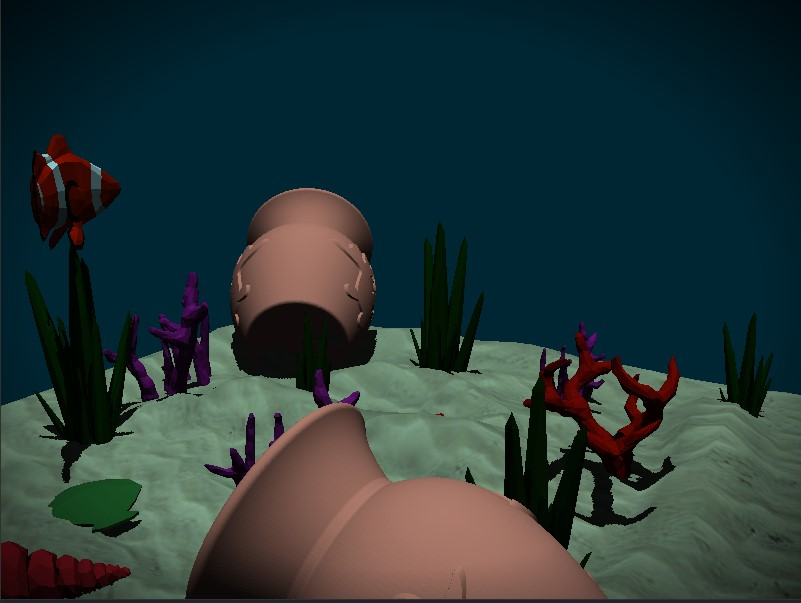
\includegraphics[width=0.32\linewidth]{imgs/base_scene.jpg}\label{fig:base_scene}
  }
  \hfill
  \subfloat[Scene with watercolor effects.]{
      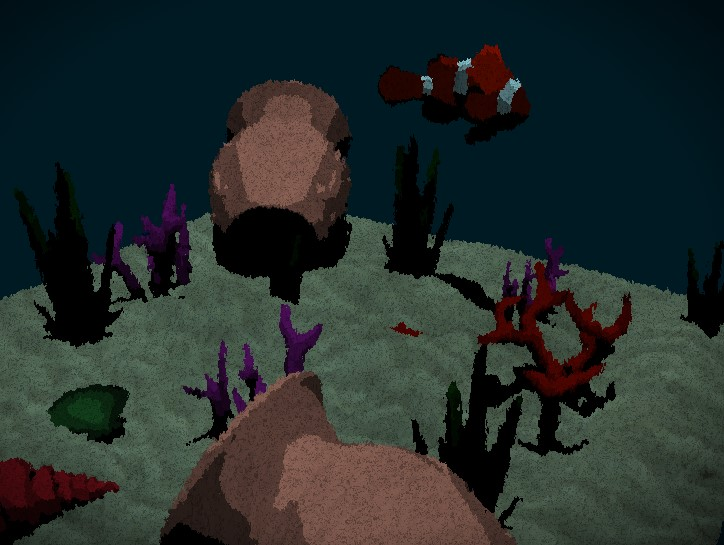
\includegraphics[width=0.32\linewidth]{imgs/watercolor_scene.jpg}\label{fig:watercolor_scene}
  }
  \hfill
  \subfloat[Final scene with all effects.]{
      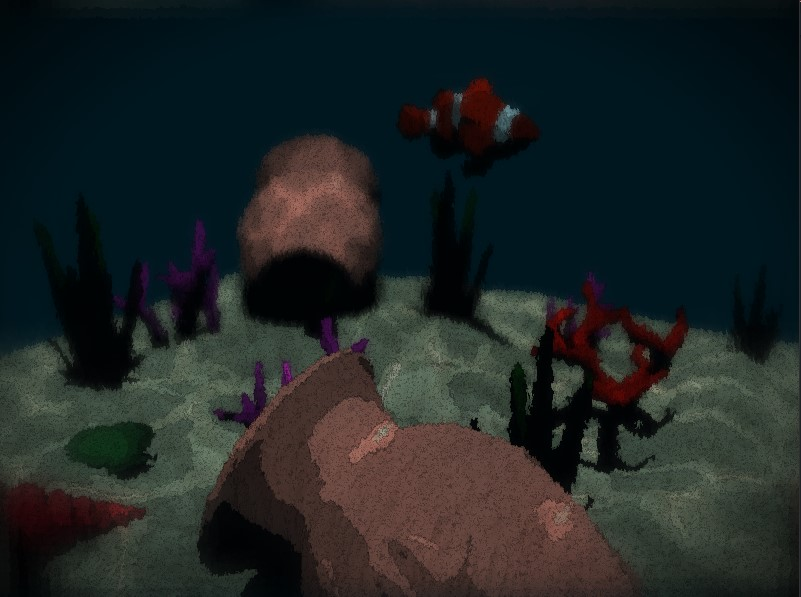
\includegraphics[width=0.32\linewidth]{imgs/all_scene.jpg}\label{fig:all_scene}
  }
  \caption{Final underwater scene with multiple levels of effects.}
  \label{fig:project_results}
  \end{figure}
}
\makeatother
\maketitle

\begin{abstract}
Watercolor rendering is a unique non-photorealistic rendering (NRP) technique, 
used to simulate hand painting art on a 3D scene. In this paper, we attempt to
combine the effects of watercolor rendering with additional caustics and underwater
effects in order to produce an abstract scene with a swimming fish in OpenGL. 
Figure \ref{fig:project_results} shows the resulting scene with various levels of effects applied.

\end{abstract}

\section{Introduction}
\label{sec:introduction}

The use of watercolor in the 3D industry is rare and usually limited to static images. 
It  goes again the general trend to make environments more realistic and detailed. This unique style, 
on the other hand, allows for some interesting variations of saturation and brightness, as well as vibrant, 
eye-catching colors that no other medium can match. Creating pleasant watercolor results requires 
careful planning, as well as a great deal of artistic understanding and experience. \medskip \par

\noindent
When used properly, this mix of bright, dancing colors and textured brush strokes creates images that appear 
simple at first glance, while retaining a surprising amount of details. As such, this style is often used in
architectural visualisation to produce rich images that allow for a quick understanding of the content, as can 
be seen in Figure \ref{fig:watercolor_architecture}.

\begin{figure}[h]
    \centering
    \subfloat[Dark, narrow street in \centering London.]{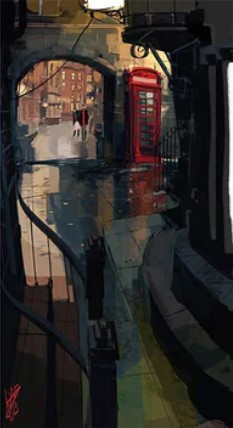
\includegraphics[width=0.4\columnwidth]{imgs/watercolor_architecture.jpg}\label{fig:f1}}
    \hfill
    \subfloat[Ponte San Angelo \centering ©Gerald Fritzler.]{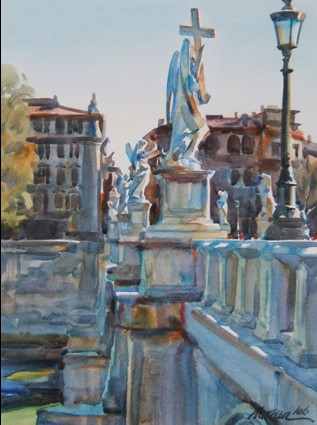
\includegraphics[width=0.4\columnwidth]{imgs/watercolor_architecture_2.jpg}\label{fig:f2}}
    \caption{Watercolor style for architectural visualisation}
    \label{fig:watercolor_architecture}
\end{figure}

\noindent
Please note, however, that these examples were produced in a watercolor style that differs from the one 
presented in this paper.

\medskip \par
\noindent
Our main inspiration for this work comes from our wish to experiment with cel shading in an underwater 
scenery. While looking for reference material, we stumbled upon a relevant video that implement
this effect using Blender \cite{caustics_video}. We decided to push the idea further by mixing in a watercolor
effect as additional passes on top using a paper from \cite{watercolor_paper}.

\begin{figure}[h]
    \centering
    \subfloat[]{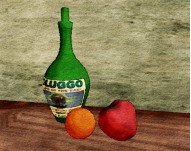
\includegraphics[width=0.45\columnwidth]{imgs/wp_result_1.jpg}\label{fig:wp1}}
    \hfill
    \subfloat[]{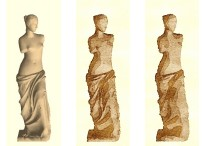
\includegraphics[width=0.45\columnwidth]{imgs/wp_result_2.jpg}\label{fig:wp2}}
    \caption{Some results from the reference watercolor paper.}
    \label{fig:watercolor_architecture}
\end{figure}

\medskip \par
\noindent
In this paper, we present a brief overview of the scene content, and project framework. 
We then go over the general pipeline used to produce the results in Figure \ref{fig:project_results}, before
diving into the implementation details of each step in their specific section. Lastly, some interesting 
results and research discussion will be mentionned, before concluding.

\section{Scene}

\subsection{Framework}

The source code for the project can be found on Github \cite{watercolor_underwater}. 
The code was written in C++ with OpenGL 4.6 core. We've used the LearnOpenGL \cite{learnopengl} 
online resource to bootstrap some of the initial work (camera class, shader class, model loading).

\subsection{Content}
The scene models an underwater environment with multiple static low polygon meshes scattered around. 
The floor is made of a square displaced patch produced in Blender, with a sand texture on top. 
All objects used in this project were not modeled by us, and are available for free on CgTrader \cite{cgtrader}.

\medskip \par
\noindent
In addition, an animated low polygon fish is placed in the water above. 
Only the sand plane model is textured, all other models use a constant color per face. 
Figure \ref{fig:scene_content} shows the models of the underwater scene without any effect applied on them.

\begin{figure}[h]
    \centering
    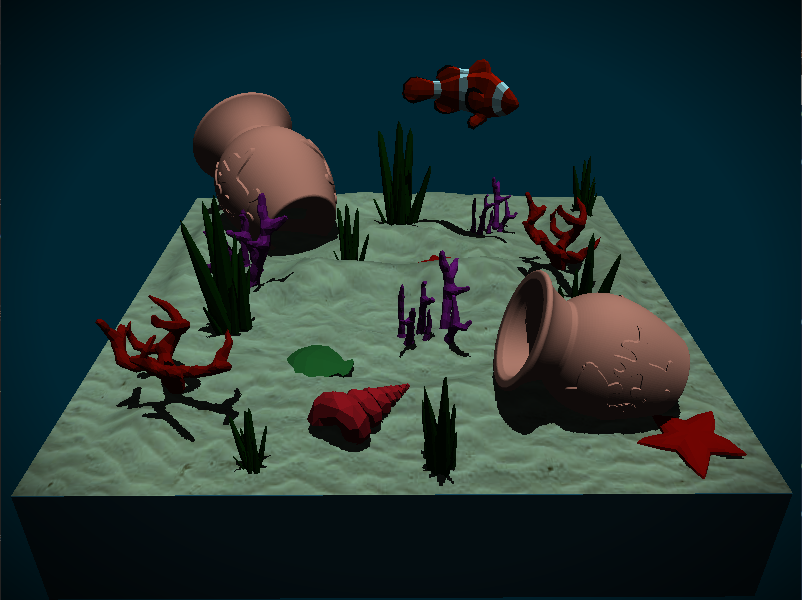
\includegraphics[width=.9\columnwidth]{imgs/scene_contents.png}
    \caption{Content of the scene with diffuse light.}
    \label{fig:scene_content}
\end{figure}

\begin{figure}[h]
    \centering
	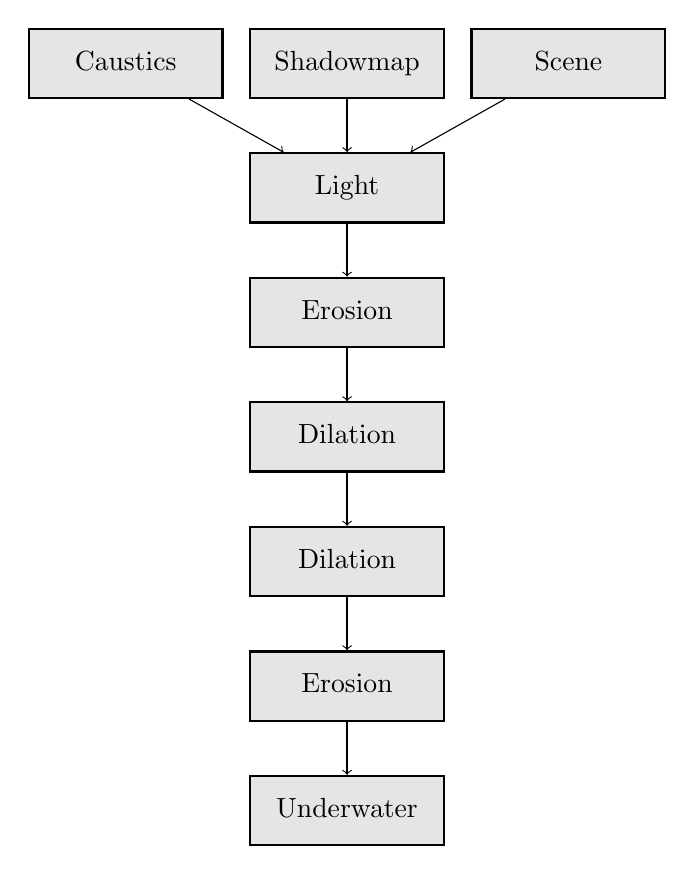
\begin{tikzpicture}[
	renderpass/.style={rectangle, draw=black, fill=black!10, thick, minimum height=2.5em, minimum width=7em, text height=height{"A"},text depth=depth{"g"}},
	]
	\node[renderpass] at (0, 0) (caustics) {Caustics};
	\node[renderpass] at (8em, 0) (shadowmap) {Shadowmap};
	\node[renderpass] at (16em, 0) (scene) {Scene};
	
	\node[renderpass] at (8em, -1 * 4.5em) (light) {Light};
	\node[renderpass] at (8em, -2 * 4.5em) (erode) {Erosion};
	\node[renderpass] at (8em, -3 * 4.5em) (dilate) {Dilation};
	\node[renderpass] at (8em, -4 * 4.5em) (dilate2) {Dilation};
	\node[renderpass] at (8em, -5 * 4.5em) (erode2) {Erosion};
	\node[renderpass] at (8em, -6 * 4.5em) (underwater) {Underwater};
	
	\draw[->] (caustics) to (light);
	\draw[->] (shadowmap) to (light);
	\draw[->] (scene) to (light);
	\draw[->] (light) to (erode);
	\draw[->] (erode) to (dilate);
	\draw[->] (dilate) to (dilate2);
	\draw[->] (dilate2) to (erode2);
	\draw[->] (erode2) to (underwater);
	\end{tikzpicture}
	\caption{Schema of all the render passes in the program.}
	\label{fig:render_passes}
\end{figure}

\subsection{Pipeline}

In order to draw an underwater scene, multiple effects must be combined together. 
This section provides an overview of the rendering pipeline of the project, 
and explains how each effect has been integrated in the pipeline. 
For more information about a specific effect, refer to one of the sections below.

\medskip \par
\noindent
Three main effects are added to the scene, and in addition, a very simple shadow map adds some realism. 
The main effects are enumerated below.
\begin{enumerate}
	\item Caustics
	\item Shadow map
	\item Watercolor rendering
	\item Underwater effects
\end{enumerate}

\noindent
The ordering of all render passes is shown in figure~\ref{fig:render_passes}. 
Note that a render pass is defined by a series of draw calls that render to a given target. 
In our case, all render passes except the last one render to framebuffers. 
The correspondence between render passes and the corresponding effects is described below.

\medskip \par
\noindent
The caustic effect (further described in section~\ref{sec:caustics}) works as follows: 
it renders a caustic texture on a framebuffer and then projects the texture on the scene. 
This effect therefore requires a separate pass and a dedicated framebuffer for the texture to be rendered in.

\begin{figure*}[h]
    \centering
    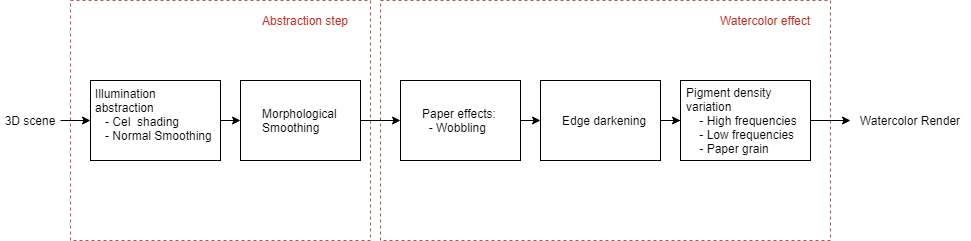
\includegraphics[width=.9\linewidth]{imgs/watercolor_pipeline.png}
    \caption{Simplified watercolor pipeline.}
    \label{fig:watercolor_pipeline}
\end{figure*}

\bigskip \par
\noindent
The shadowmap works in much the same way, it renders a depth buffer in the point of view of the light, 
and then a check is made when drawing the light (note that the caustics are part of the light) 
to see if a given fragment is illuminated or not. Our shadow map implementation is very simple, 
and does not do a lot of work to obtain good-looking shadows. In practice, the watercolor effect 
is very prominent, so the irregularities are not very visible.

\medskip \par
\noindent
The caustic texture and the shadow map are applied on the scene in a separate pass, the "Light" pass. 
We use deferred rendering to calculate the illumination of the scene, so the light pass requires the position, 
normals and base colors for every fragment of the scene. 
The "Scene" pass is responsible for drawing all objects of the scene in order to retrieve the position, 
normal and color information per pixel and send it to the light pass.

\medskip \par
\noindent
The watercolor effect (further described in section~\ref{sec:watercolor}) is a bit more complicated. 
In order to be able to correctly apply the effect, we need to be able to sample neighbouring pixels. 
In order to achieve this, the effect is split over multiple passes. Following the light pass, 
4 passes perform alternating erosion and dilation effects. 
Then, the rest of the watercolor effect is applied at the same time as the underwater effects, 
in the underwater pass.

\medskip \par
\noindent
Finally, the underwater effect (further described in section~\ref{sec:underwater}) is applied at 
the end of the pipeline, in the underwater pass. The underwater effect is therefore computed in 
the same shader as the end of the watercolor effect. The result is rendered directly on the screen 
and completes the render pipeline.

\section{Watercolor rendering}
\label{sec:watercolor}

As mentionned in Section~\ref{sec:introduction}, we have based our watercolor implementation on a paper by 
\cite{watercolor_paper}, with a few modifications to accomodate for the underwater scene context. 
In this section,we will present the pipeline proposed by the authors to produce the desired effect, 
as well as the areas where our implementation deviates from the original paper. 

\medskip \par
\noindent
Figure \ref{fig:watercolor_pipeline} shows a simplified version of the pipeline, with only a 3D scene as input, 
as opposed to a 3D scene or static image used by the authors. We also got rid of the dry brush effect, as it 
was conflicting with the desired underwater effect.

\subsection{Cel shading}

The first modification needed for a watercolor effect is to lower the amount of details available 
in the image by reducing the color variations. On a static image, a color segmentation step, through the use
of a mean shift algorithm, would be required to obtain the desired density. In this case however, using the 
light position and fragment normals, we can achieve good results with a simple cel shader combined with 
normal smoothing.

\medskip \par
\noindent
For the cel shading, we compute the color of each fragment using a simple diffuse model. 
We can then transform that rgb color to hsv space in order to access its color intensity value. 
Through its hsv representation, the color intensity can be clamped to a chosen level using the formula
presented in Figure \ref{fig:celshading_levels}. 
Doing so clamps the intensity value to 4 different levels, while preserving the overall color.

\lstinputlisting{code/celshading.cpp}

\vspace{-1.5em}

\begin{figure}[h]
    \centering
    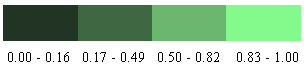
\includegraphics[width=.8\columnwidth]{imgs/celshading_levels.png}
    \caption{Cel shading color transitions for the green color.}
    \label{fig:celshading_levels}
\end{figure}

\vspace{-1.5em}

\begin{figure}[h]
    \centering
    \subfloat[Diffuse shading.]{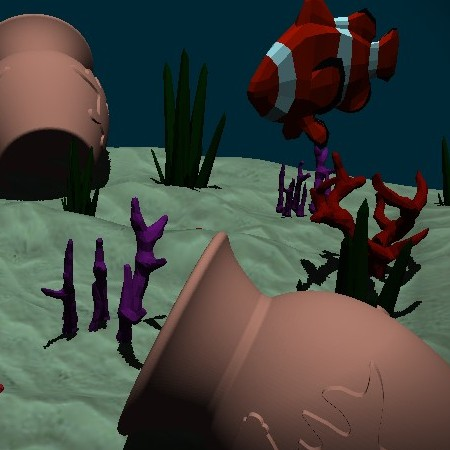
\includegraphics[width=0.47\columnwidth]{imgs/diffuse_shading.jpg}\label{fig:dshading}}
    \hspace{1em}
    \subfloat[Cel shading.]{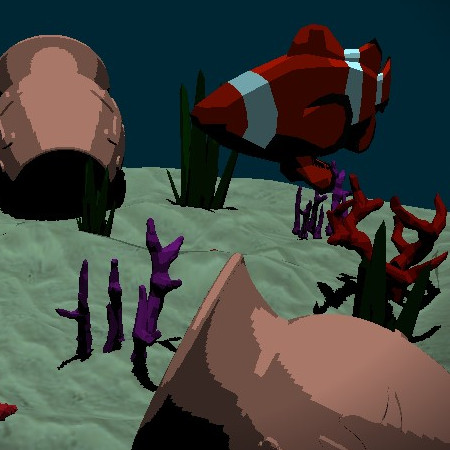
\includegraphics[width=0.47\columnwidth]{imgs/cel_shading.jpg}\label{fig:cshading}}
    \caption{Diffuse vs cel shading with low poly models.}
    \label{fig:celshading_result}
\end{figure}

\subsection{Normal smoothing}

As can be seen in Figure \ref{fig:celshading_result}, when used on low poly models with curved surface,
such as the clay pot, it results in aliasing in the transitions between the levels. To fix that, as well as
reduce some additionnal detail in the shape, we use a process called normal smoothing.

\medskip \par
\noindent
Normal smoothing consists of average every vertex normal with its neighbors' normals. Each pass reduce 
the amount of details in the model, while preserving the overall silhouette intact.
The process can be repeated multiple time in order to obtain the desired level of details, 
or lack of, in this case.

\begin{figure}[h]
    \centering
    \subfloat[Cel shading, no smoothing.]{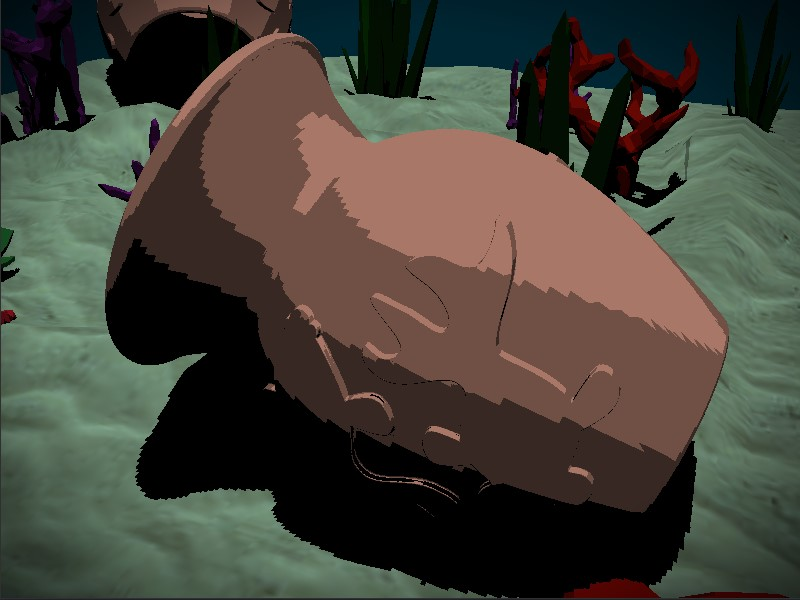
\includegraphics[width=0.47\columnwidth]{imgs/normal_smoothing_0.jpg}\label{fig:nsmoothing0}}
    \hspace{1em}
    \subfloat[1 pass of smoothing.]{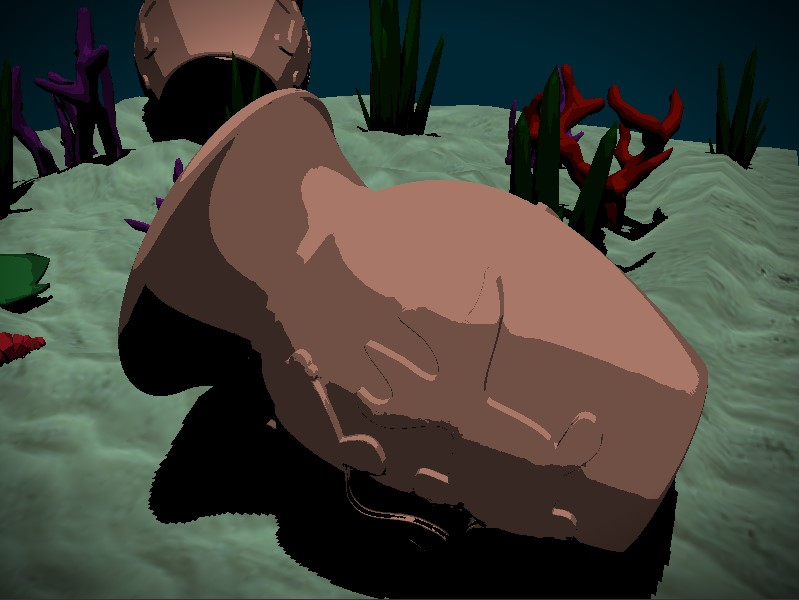
\includegraphics[width=0.47\columnwidth]{imgs/normal_smoothing_1.jpg}\label{fig:nsmoothing4}} \\
    \subfloat[7 passes of smoothing.]{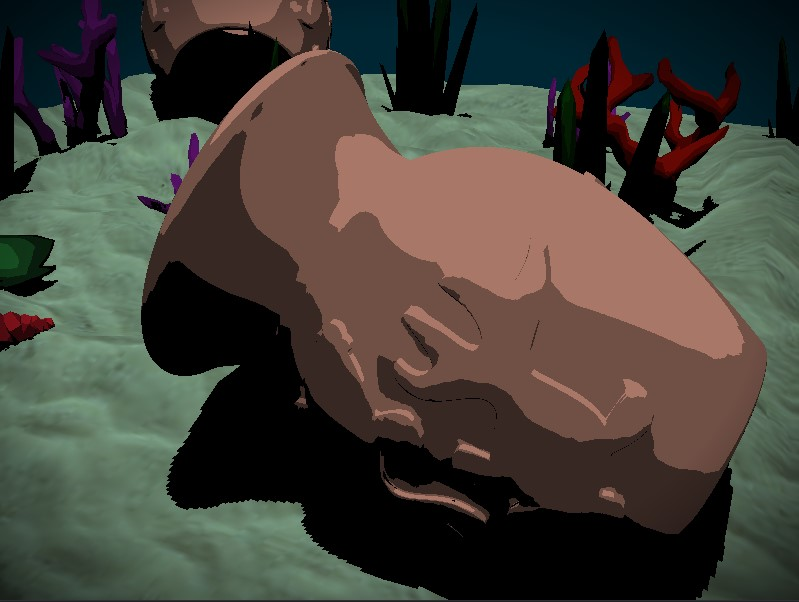
\includegraphics[width=0.47\columnwidth]{imgs/normal_smoothing_7.jpg}\label{fig:nsmoothing7}}
    \hspace{1em}
    \subfloat[20 passes of smoothing.]{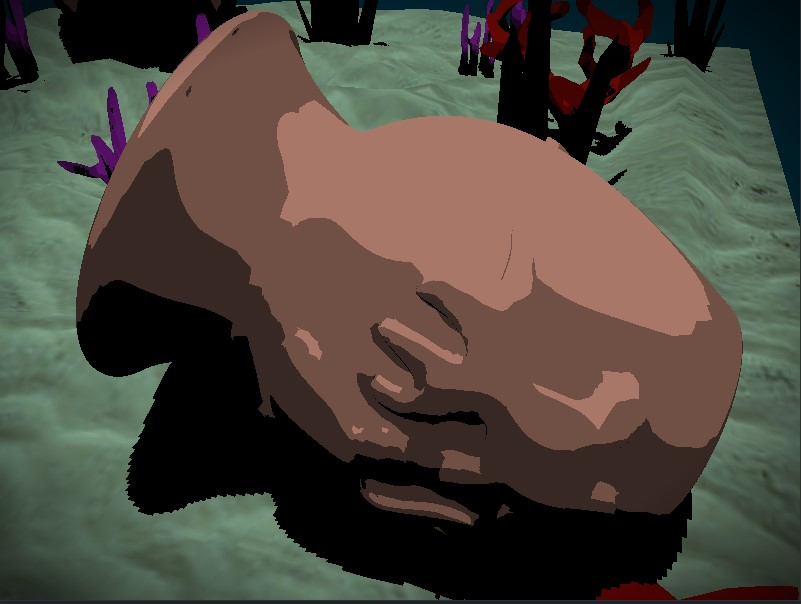
\includegraphics[width=0.47\columnwidth]{imgs/normal_smoothing_20.jpg}\label{fig:nsmoothing20}}
    \caption{Effect of normal smoothing on the cel shading.}
    \label{fig:normal_smoothing_results}
\end{figure}

\noindent
Figure \ref{fig:normal_smoothing_results} shows various level of normal smoothing applied to the pot. 
We have found that repeating the process a total of 7 times gives the best results across a variety of models,
and have kept that for the rest of the experiment.

\medskip \par
\noindent
The initial implementation was done in a fragment shader, using a deferred rendering technique to query the 
neighboring fragment normals using a post process normal map. The issue with this approach was that we could 
only do one pass per fragment shader, and that was repeated every frame. To get 7 passes using this technique, 
we would have to write the normals to a texture and do a pass with the post process shader multiple times every 
frame.

\medskip \par
\noindent
As a tradeof, in order to save rendering time, we've instead decided compute the normal smoothing on a per vertex basis, on
the CPU at load time. This only happens at the beginning of the program once, and can easily be repeated any 
number of time necessary. The issue however, is that it is done on the CPU, and can slow down considerably the 
program if a large number of detailed models is used. 

\medskip \par
\noindent
In the context of this experiment, the additional load time at the opening of the program was not an issue 
given the small amound of low poly models used.

\subsection{Morphological smoothing}

An additionnal morphological smoothing pass can be applied on the resulting image to further reduce the level
of details in the scene. Just like most of the other watercolor steps, they are applied on a post-process basis.
We've decided to apply it in this case as it helps reducing the sharp noise introduced by the wobbling to an
acceptable range, as the reminder of the noise is necessary to obtain the desired watercolor effect.

\medskip \par
\noindent
The smoothing we've applied is composed of an initial opening sequence (Erosion - Dilation) followed by a closing sequence
(Dilation - Erosion). Erosion consists of applying a kernel over a black and white image, and setting the target
fragment to 1 if every fragment in the kernel is also 1 (white). Dilation is the opposite operation, it sets a fragment
to 1 if at least one fragment in the kernel is 1. 

\begin{figure}[h]
    \centering
    \subfloat[Opening sequence.]{
\includegraphics[width=0.47\columnwidth]{imgs/opening.png}\label{fig:opening}}
    \hspace{1em}
    \subfloat[Closing sequence.]{
\includegraphics[width=0.47\columnwidth]{imgs/closing.png}\label{fig:closing}}
    \caption{OpenCV documentation on morphological operations.}
    \label{fig:opencv-morph}
\end{figure}

\noindent
A difficulty arise when dealing with colored images: What do we define as 0 and 1 respectively? 
Since images are not black and white, each pixel queried by the kernel is likely to be slightly different, 
and both operations cannot be applied as is. Another consideration is that the morphological operation 
should not introduce new colors to the image, as the goal is to reduce the amount of details, not increase it.

\medskip \par
\noindent
A possible solution for that is to use a gray-scaled approach to the morphological smoothing, and process each
r, g and b channels individually. Alternatively, the smoothing could be applied to the value part on the HSV 
space of the image. Both of those approach break the color preservation criterion. 
\cite{morph_colors_1} perform more advanced operations on the chromatic scale, by mixing the reduced 
and conditional ordering of the underlying image. 
\cite{morph_colors_2} construct a specific color ordering for each particular image and perform morphological 
operations using this ordering.

\medskip \par
\noindent
Such extended approaches were not needed in the scope of this experiment, as the morphological smoothing serves
as an additional polish between the normal smoothing and the wobbling effect. For this reason, we've settled on 
a simple, straightforward solution. 

\medskip \par
\noindent
A 3x3 kernel is applied over the image, with each r, g and b channel being processed independently. For the 
erosion operation, the lowest channel value in kernel is taken as the fragment's channel value. 
For the dilation, it's the opposite, the highest channel value is kept.

\begin{figure}[h]
    \centering
    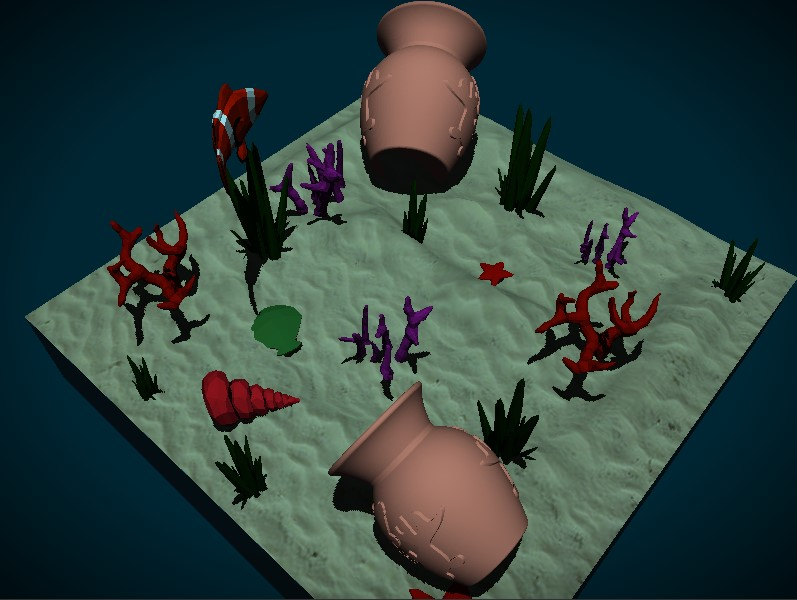
\includegraphics[width=\columnwidth]{imgs/no_smoothing_2.jpg}
    \caption{No morphological smoothing.}
    \label{fig:no_ms}
\end{figure}

\begin{figure}[h]
    \centering
    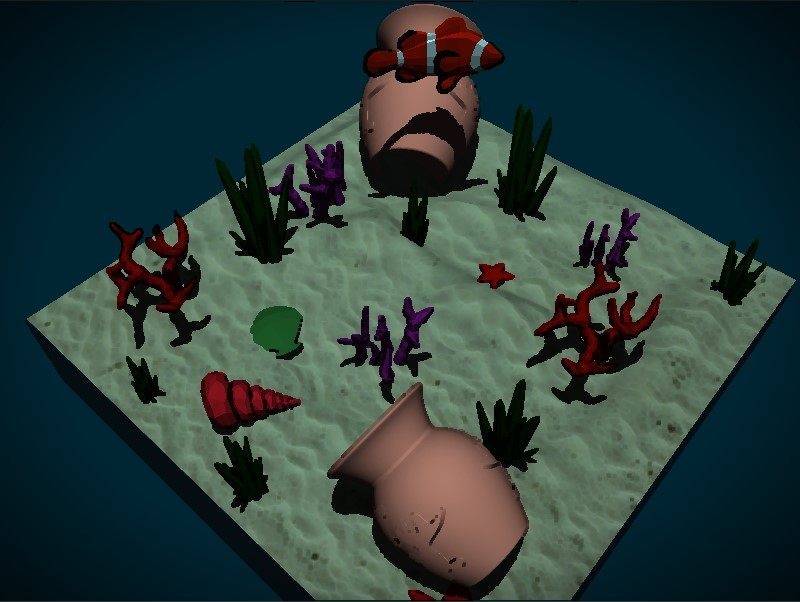
\includegraphics[width=\columnwidth]{imgs/erosion.jpg}
    \caption{Single pass erosion effect.}
    \label{fig:erosion_ms}
\end{figure}

\begin{figure}[h]
    \centering
    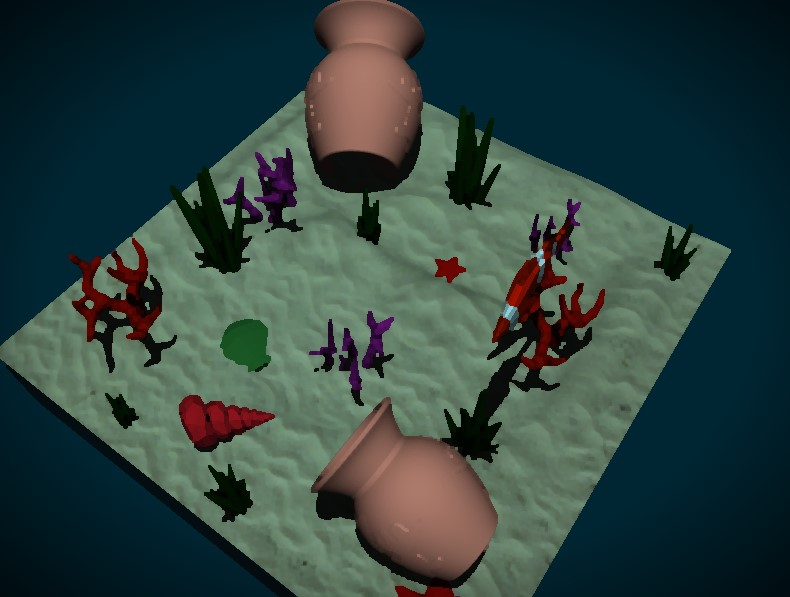
\includegraphics[width=\columnwidth]{imgs/opening_closing.jpg}
    \caption{Full opening-closing sequence.}
    \label{fig:opening_closing_ms}
\end{figure}

\begin{figure}[h]
    \centering
    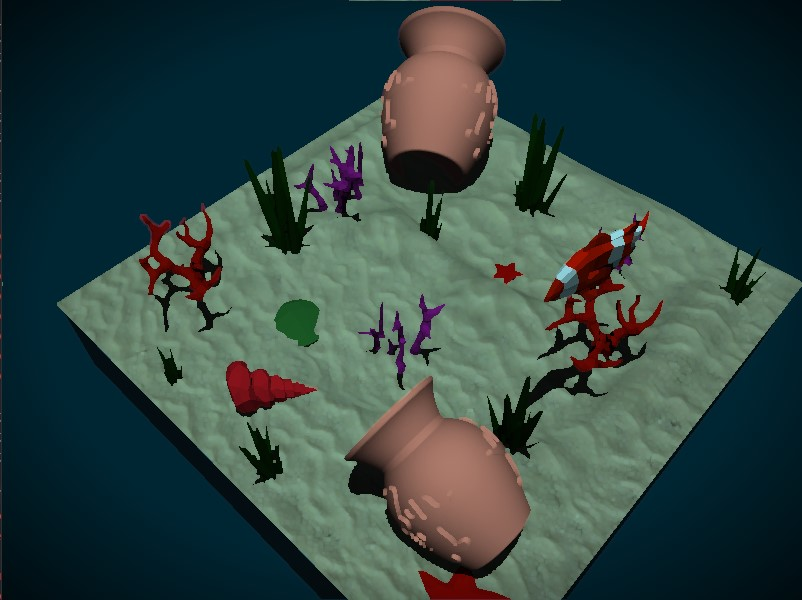
\includegraphics[width=\columnwidth]{imgs/dilation.jpg}
    \caption{Single pass dilation effect.}
    \label{fig:dilation_ms}
\end{figure}

\newpage
\noindent
Figures \ref{fig:no_ms} and \ref{fig:opening_closing_ms} show an overview of the scene, before and after 
applying the morphological sequence. Due to the small sequence that was used, only a little bit of the 
details around some edges were smoothed out. Using a bigger kernel, and possibly a different approach to 
the smoothing could yield better results. 

\medskip \par
\noindent
Figures \ref{fig:erosion_ms} and \ref{fig:dilation_ms} show the result of each operation. 
Erosion expand and darken the edges around the objects. It can be used in conjonction with the edge darkening 
effect used later on in the pipeline. Dilation, on the other hand, 
lighten the edges and make the objects thinner.

\subsection{Wobbling effect}
In order to simulate the displacement of paint due to the paper height, a wobbling effect needs to be added. The wobbling effect consists in displacing fragments along the viewport, based on the paper height.

\medskip \par
\noindent
In practice, in order to get the horizontal and verical displacement of the pixel, the gradient of the paper height is used. To compute the gradient, the finite element method is used. The following code listing shows how the gradient of the paper height map:
\lstinputlisting{code/wobbling-effect.glsl}

\medskip \par
\noindent
Here the \verb|paper| texture corresponds to the height of the paper. This was obtained by using pictures of paper. The \verb|wobFactor| variable is a parameter that is adjusted depending on the texture so that it corresponds to the difference between two pixels. Once the paper gradient is computed, the fragments position is changed based on the gradient (multiplied by a parameter to control the intensity of the effect). This is done by adjusting the coordinates at which the fragment is sampled (\verb|vertTexCoord|).

\medskip \par
\noindent
Figure \ref{fig:wobbling_results} shows the effect of the wobbling on the scene. Adding the wobbling effect makes the edges of the object in particular sand out, and is not very visible inside the object, since the color is fairly constant. In addition, when the wobbling effect is used along the morphological smoothing, the morphological smoothing effect diminished the intensity of the wobbling effect.

\begin{figure}[h]
	\centering
	\subfloat[No effects.]{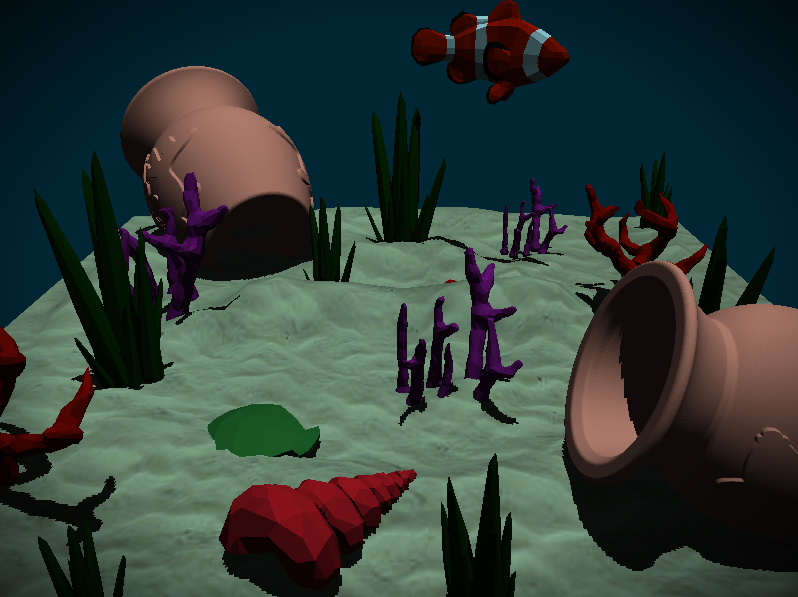
\includegraphics[width=0.47\columnwidth]{imgs/wob_off.png}\label{fig:wobbling_results0}}
	\hspace{1em}
	\subfloat[Wobbling effect.]{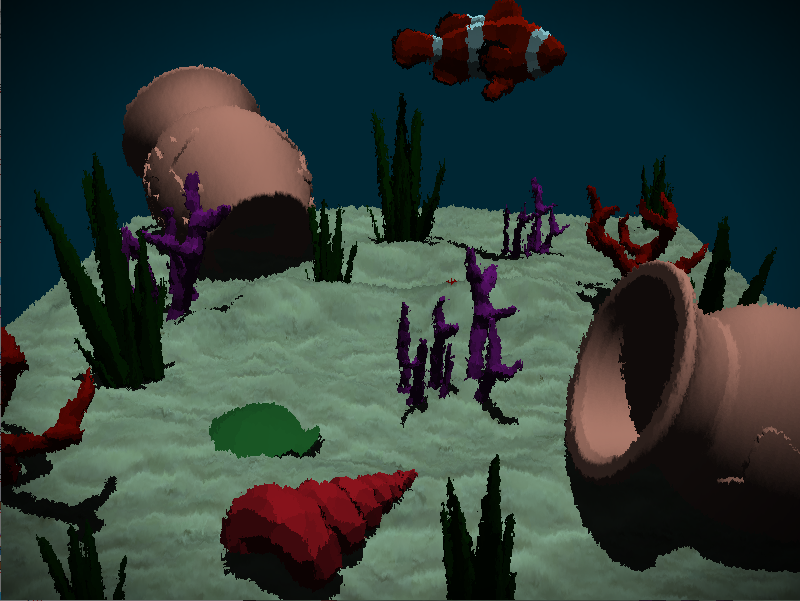
\includegraphics[width=0.47\columnwidth]{imgs/wob_on.png}\label{fig:wobbling_results1}} \\
	\subfloat[Wobbling and morphological smoothing.]{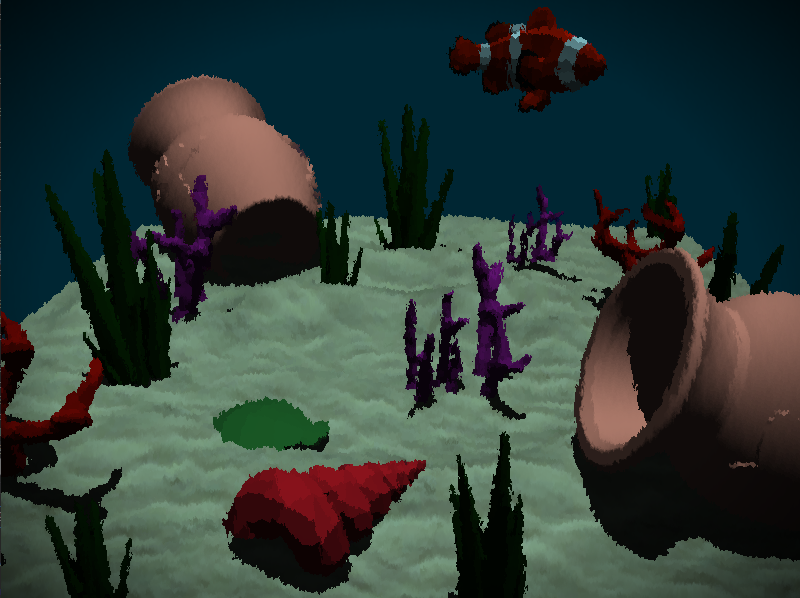
\includegraphics[width=0.47\columnwidth]{imgs/wob_on_smooth.png}\label{fig:wobbling_results2}}
	\hspace{1em}
	\caption{Effect of wobbling.}
	\label{fig:wobbling_results}
\end{figure}

\newpage~\newpage
\subsection{Edge darkening}

\begin{figure}[h]
    $$
    \begin{bmatrix}
        1 & 1 & 1\\
        1 & -8 & 1 \\
        1 & 1 & 1
    \end{bmatrix}
    $$
    \caption{Sobel 3x3 kernel.}
    \label{fig:sobel}
\end{figure}
\vspace{-0.5em}

\noindent
A simple sobel filter (Figure \ref{fig:sobel}) is applied over the image during the underwater pass 
to detect edges and darken them. We initially set the fragments with a color length, computed as the simple
vector length of the rgb color, of over 0.9 to black. The effect was however too strong, and while it was quite
aesthetically pleasant, it did not match the watercolor context.
\vspace{-0.5em}

\begin{figure}[h]
    \centering
    \subfloat[No edge darkening.]{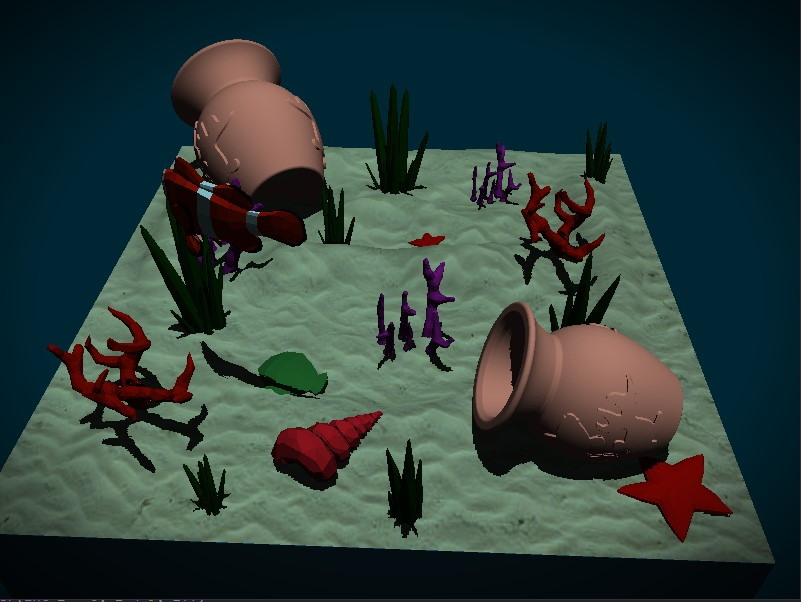
\includegraphics[width=0.47\columnwidth]{imgs/no_edges.jpg}\label{fig:no_edges}}
    \hspace{1em}
    \subfloat[Initial edge darkening.]{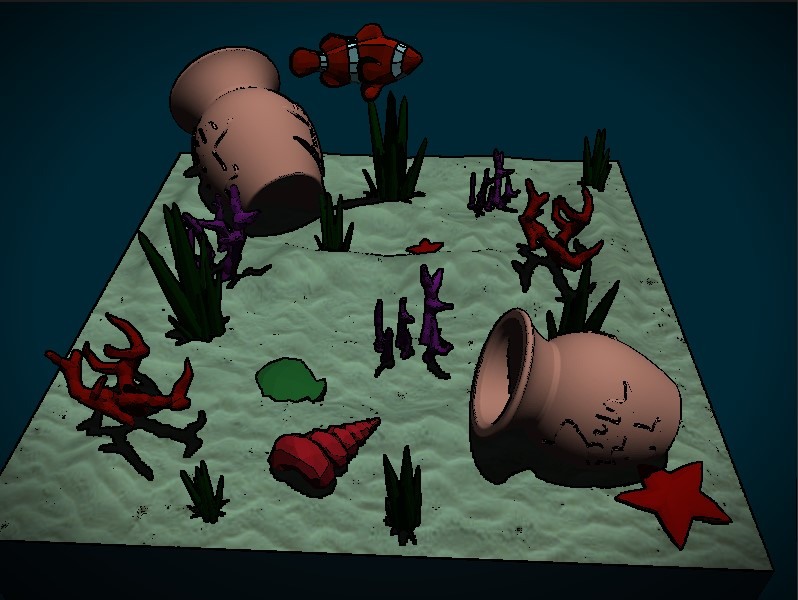
\includegraphics[width=0.47\columnwidth]{imgs/black_edges.jpg}\label{fig:initial_darken}}
    \caption{OpenCV documentation on morphological operations.}
    \label{fig:initial_edge_darkening}
\end{figure}
\vspace{-0.5em}

\noindent
Instead, the new approach was to apply a factor of 0.7 to the intensity value of the fragment in the hsv space.
This results in darkening the edges juste enough for it to be noticeable, without being too strong either. 
The darkening factor can also be tweaked depending on the needs.

\begin{figure}[h]
    \centering
    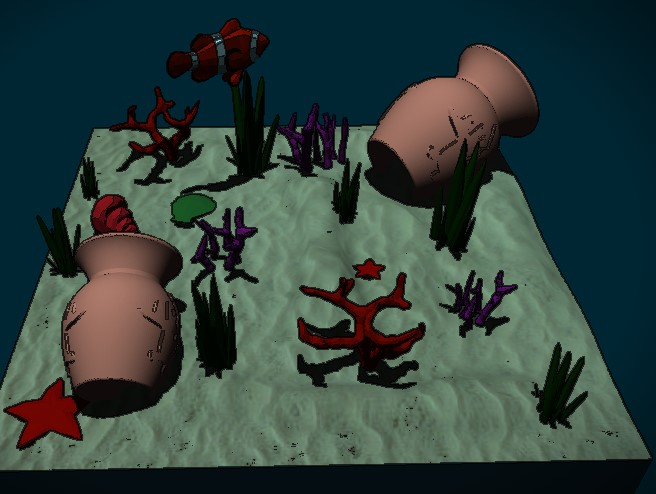
\includegraphics[width=.9\columnwidth]{imgs/post_edge_darkening.jpg}
    \caption{Final edge darkening effect.}
    \label{fig:post_edge_darkening}
\end{figure}
\vspace{-0.5em}

\noindent
An issue with the current approach is that, since the edge darkening is handled in the underwater pass,
the image~already contains the caustics from the light pass. As such, using a strong edge darkening results 
in the transition between water and light being darkened as well, which is undesirable. Moving that step back 
to the light pass would interfer with the morphological smoothing. 
A solution to this is mentionned in Section \ref{sec:future_work}.

\newpage
\subsection{Pigment density variation}

TODO: Talk about pigment density variation here.

\newpage
\section{Caustics}
\label{sec:caustics}

In order to render caustics, we use a method called Periodic Caustic Textures \cite{periodic_caustic_textures}. 
This method is relatively simple, and the biggest advantage over other methods (for instance rendering caustics 
using photon mapping \cite{caustics_photon_mapping}) is that it is easy to implement and not very 
computationally expensive. The method used also achieves good-looking results, 
compared with the GPU Gems method \cite{caustics_gpu_gems}, which we also tried to implement.

\subsection{Algorithm}
First, a grid with a certain resolution is generated. The grid is then rendered on a framebuffer. 
The vertex shader used in the rendering changes the x and y coordinates of the grid vertex by refracting 
the vertex as if it was a ray of light coming from above. The distorted mesh is then drawn in the fragment 
shader, using the ratio of the new area of a triangle over the original area of a triangle to calculate the 
color. This way, if the vertices are sent close together, the caustic color approaches white, while if the 
vertices are sent apart, the caustic color approaches black.
Figure \ref{fig:caustic_algorithm} shows a visual representation of the algorithm used to generate caustics.

\begin{figure}[h]
	\centering
	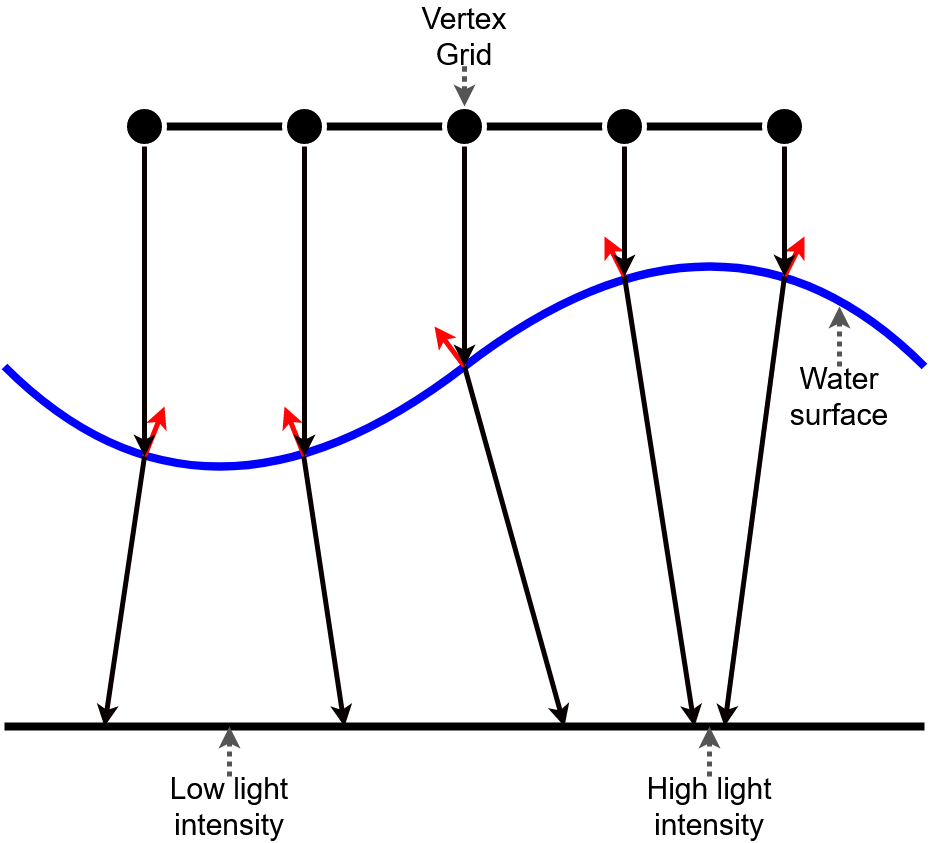
\includegraphics[width=.9\columnwidth]{imgs/caustic_algorithm.png}
	\caption{Schema of the algorithm used to generate the caustic texture.}
	\label{fig:caustic_algorithm}
\end{figure}

\noindent
With this algorithm, there is a risk that a vertex on the edge of the camera travels towards the 
inside of the viewport of the camera, leaving an unrendered section on the side of the texture. 
To prevent this, the grid is created too big (in our implementation by a factor of 1.2). 
This ensures that the texture is always rendered.

\medskip \par
\noindent
Figure \ref{fig:caustics_texture} shows the caustic texture generated by this approach. 
No that the squares of the grid are still visible by looking closely at the image despite the resolution 
of the grid being high. However, once the toon shading has run, these are no longer perceptible.

\begin{figure}[h]
    \centering
    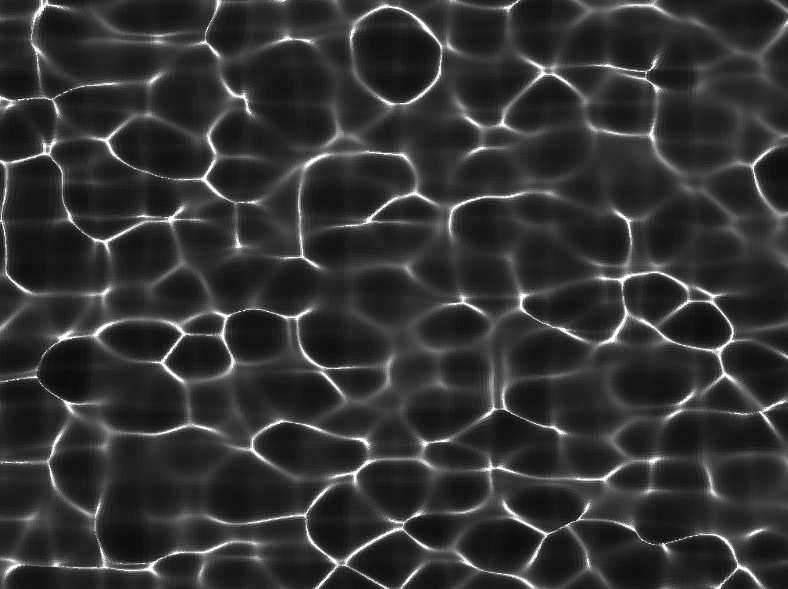
\includegraphics[width=.6\columnwidth]{imgs/caustics_texture.png}
    \caption{Caustic texture generated from our implementation.}
    \label{fig:caustics_texture}
\end{figure}

\vspace{-1em}

\subsection{Water height}
In order to generate the caustic texture, the algorithm must refract and project on the ground 
the grid vertices. This means that the algorithm needs access to a water height and a water normal 
for each vertex. We can compute the normal if we have access to the water height by using the finite 
element method. To obtain the water height, a fractal noise (in our case 3 layers of Perlin noise) is 
generated in the caustic vertex shader. In order to generate the Perlin noise, an implementation from 
Stefan Gustavson was used \cite{perlin_noise}.

\medskip \par
\noindent
To animate the water height over time, we used a 3d Perlin noise, with the time as one dimension. 
This generates unrealistic water heights, but since we only use the water height to compute the caustics, 
the end result still looks good.

\subsection{Projection on the scene}
Once the caustic texture is generated, we project the texture on the scene to give the 
impression that the scene is illuminated by the caustics. This is an approximation, 
since we assume that all light rays in the water travel vertically, but the result is good enough. 
Figure \ref{fig:scene_with_caustics} shows the scene with the caustics projected on it.

\vspace{-0.5em}
\begin{figure}[h]
    \centering
    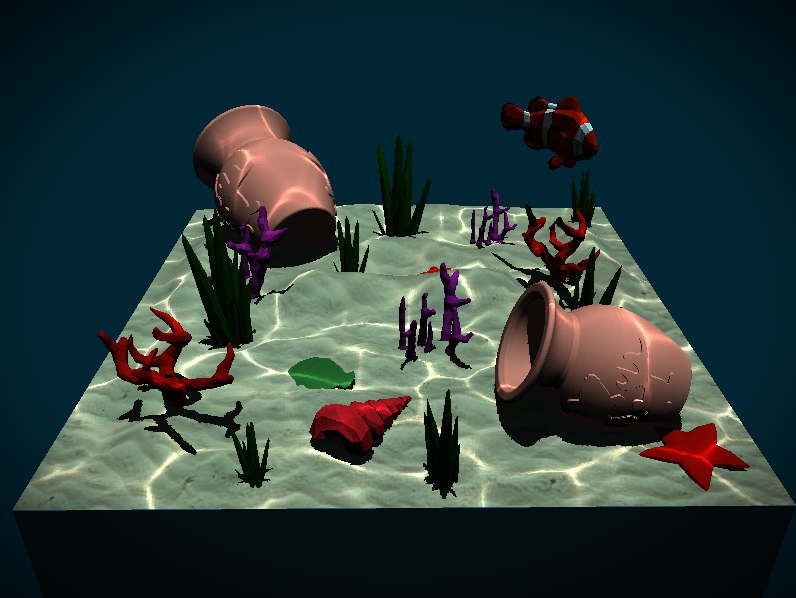
\includegraphics[width=\columnwidth]{imgs/scene_with_caustics.png}
    \caption{Scene with the projected caustic texture.}
    \label{fig:scene_with_caustics}
\end{figure}

\section{Underwater effects}
\label{sec:underwater}

In order to make the scene look like an underwater scene and make the final result more attractive, three additional effects have been implemented. These effects are not based on a physical model, but are purely cosmetic. 

\subsection{Blur}
The first effect is a blur. This simulates the blur that is seen underwater with a human eye. The blur we added is dependent on two factors, the distance of a fragment to the camera (fragments further away are blurrier), and the distance of the fragment to the center of the viewport (fragments on the side and in the corners of the viewport will be blurrier). This effect is not realistic, but still gives the feeling of an underwater scene.

\medskip \par
\noindent
In order to implement the blur underwater, a $5\times5$ Gaussian kernel was used. The kernel is scaled on the image using a range parameter in order to have different blur intensities without changing the speed of the algorithm. This kernel is convolved twice, once using a range of 3 and once using a range of 10. The result of both of these blurs is then mixed with the non-blurred color, using two factors, one dependent on the depth of the fragment and one dependent on the distance to the center of the viewport.

\medskip \par
\noindent
In order to have blur that augments fast passed a certain distance, before being used to mix the colors, 
the depth of the fragment is raised to the third power ($factor = depth^3$). 
This gives a better effect for the distance blur, as when the camera is close to an object (distance below 1), 
the blur is almost non-existent, and one the threshold is passed, the blur increases rapidly.
Figure \ref{fig:scene_with_blur} shows the scene with and without any blur.

\vspace{-1em}

\begin{figure}[h]
	\centering
	\subfloat[Without depth blur.]{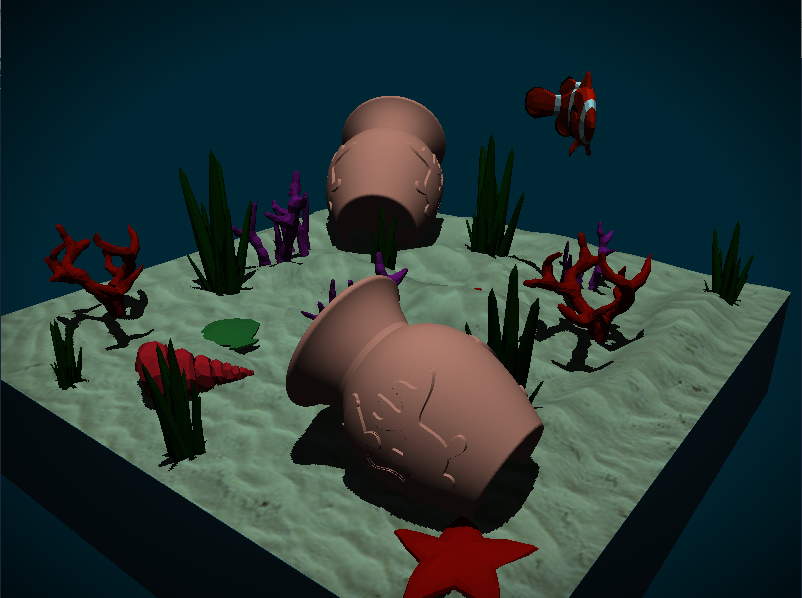
\includegraphics[width=0.47\columnwidth]{imgs/blur_off.png}}
	\hspace{1em}
	\subfloat[With depth blur.]{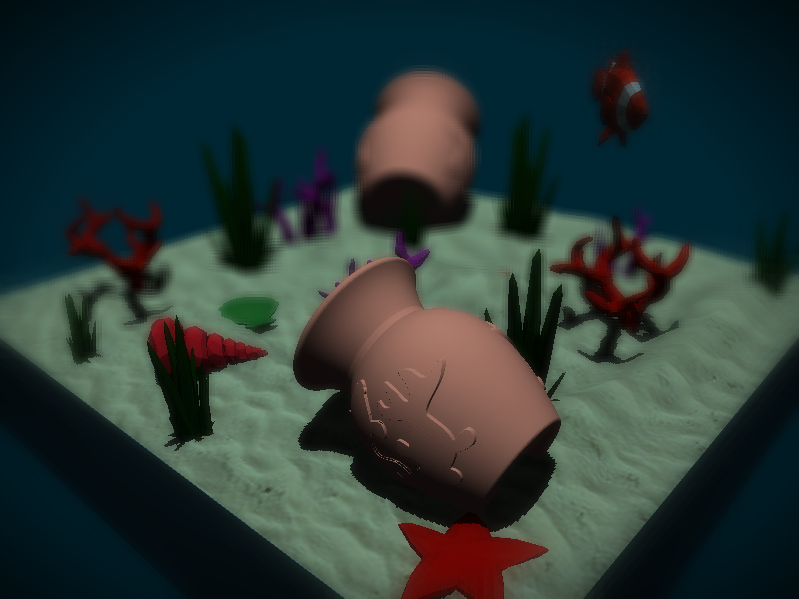
\includegraphics[width=0.47\columnwidth]{imgs/blur_on.png}}
	\caption{The effect of depth blur on the scene.}
	\label{fig:scene_with_blur}
\end{figure}

\vspace{-1em}

\subsection{Radial darkening}
The second effect is a radial darkening. This means that fragments on the edge and corners of the screen are darker. This darkening was added in order to make the end image more attractive. This is a fairly common effect, and is easy to implement. The code for the effect is shown below:
\lstinputlisting{code/radial-darkening.glsl}

\medskip \par
\noindent
Figure \ref{fig:scene_with_radial_darkening} shows the results of radial darkening on a scene. Notice the corners of the image. The effect is minimal, and can be hard to notice if it is not pointed out, but adds to the overall image attractiveness.

\begin{figure}[h]
	\centering
	\subfloat[Without radius darkening.]{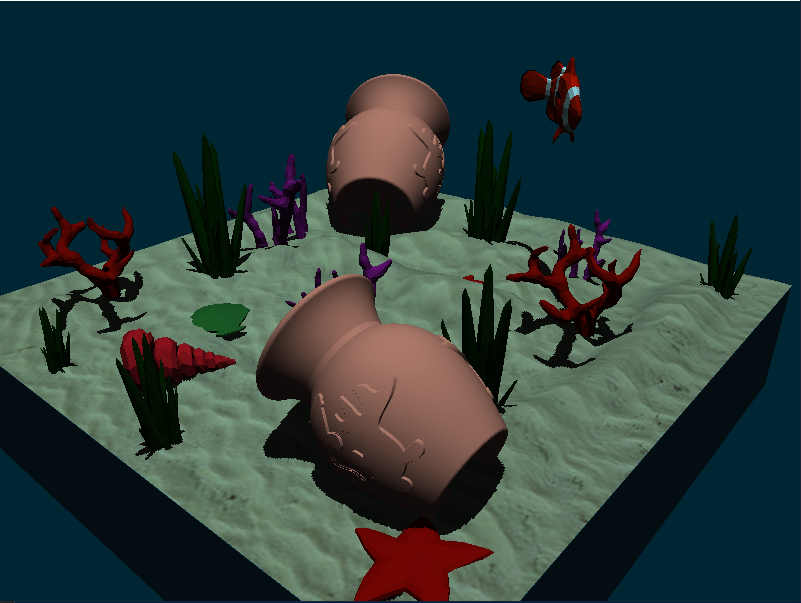
\includegraphics[width=0.47\columnwidth]{imgs/bright_sides.png}}
	\hspace{1em}
	\subfloat[With radius darkening.]{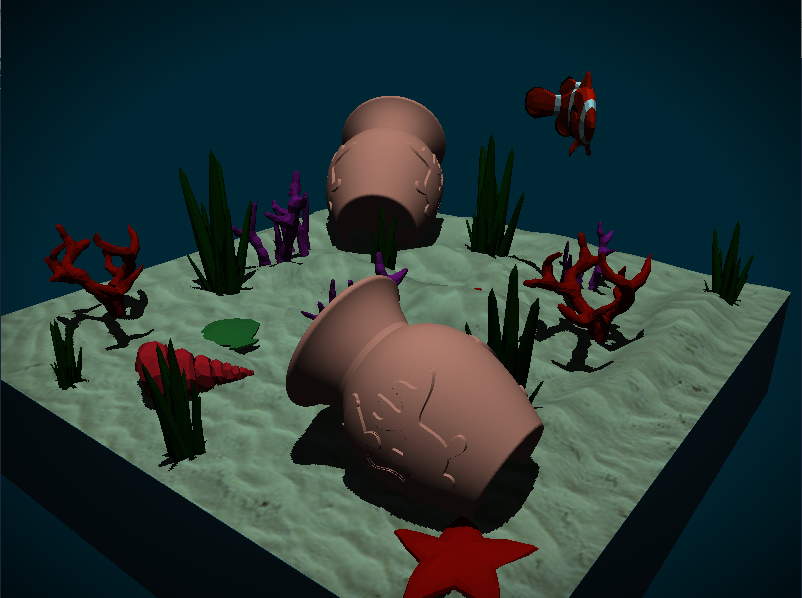
\includegraphics[width=0.47\columnwidth]{imgs/blur_off.png}}
	\caption{The effect of radial darkening on the scene.}
	\label{fig:scene_with_radial_darkening}
\end{figure}

\subsection{Color tint}
Water absorbs certain light wavelengths faster than others. In particular, red and green light are absorbed by water, so often underwater scenes take a blue tint. In order to create a similar effect, but without making it physically accurate, we tint the entire scene with a blue color.
All fragments of the scene are mixed with a color according to the following formula:
\[ color = \text{mix}\left(color, tint, 0.75\right)\]
Where tint is the tint color, defined with the rgb values $(0.0, 0.07, 0.1)$.

\medskip \par
\noindent
Figure \ref{fig:scene_with_tint} shows the effect of adding the color tint on the scene.

\begin{figure}[h]
	\centering
	\subfloat[Without tint.]{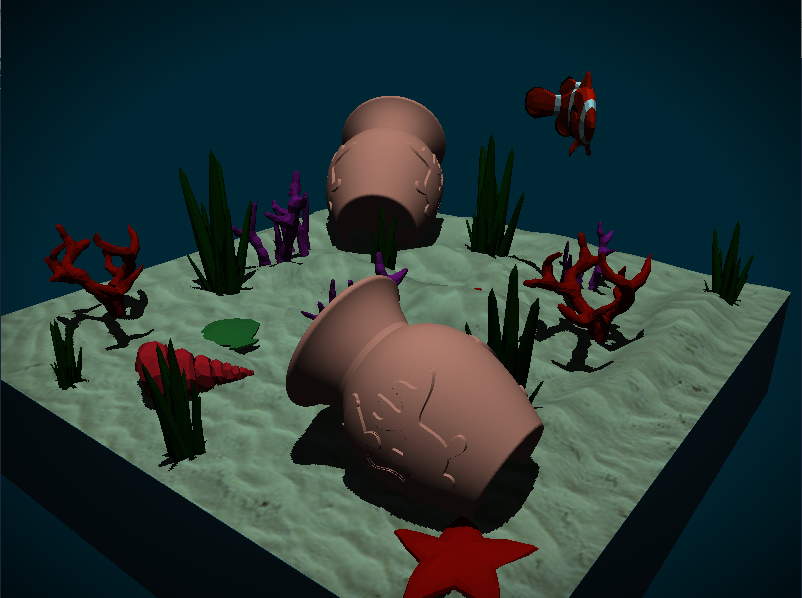
\includegraphics[width=0.47\columnwidth]{imgs/blur_off.png}}
	\hspace{1em}
	\subfloat[With tint.]{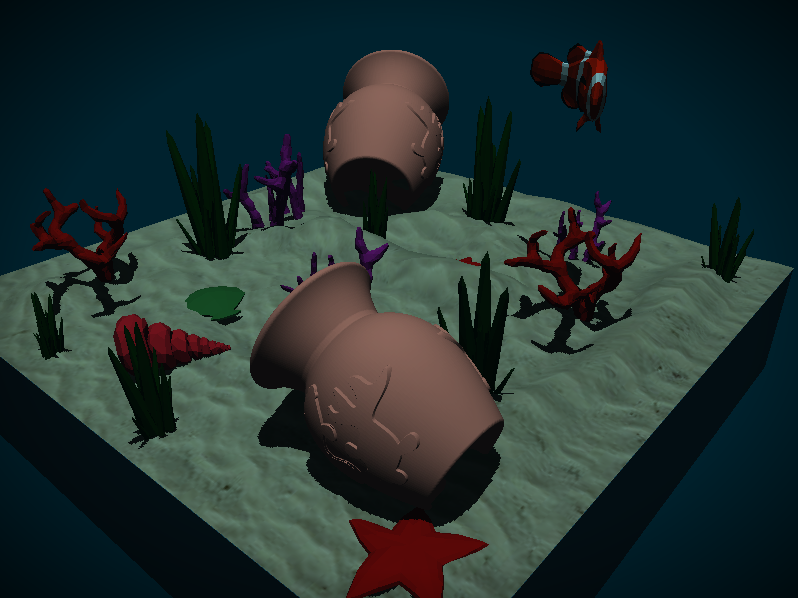
\includegraphics[width=0.47\columnwidth]{imgs/tinted.png}}
	\caption{The effect of color tint on the scene.}
	\label{fig:scene_with_tint}
\end{figure}


\medskip \par
\noindent

\section{Results}

TODO: Showcase more results here.

% \newpage
\section{Future Work}
\label{sec:future_work}
The current implementation has multiple points that could make the results better. This section outlines the major changes that could make our final result better.

\paragraph{Pigment density variation mapping in screen space.} One of the main problem of the pigment density variation effect is that to be accurate, the effect has to be applied in screen space. The problem with applying the effect in screen space is that when the objects or the camera moves, it gives the impression of a "dirty lens," and the illusion of watercolor is completely broken. To counter this effect, \cite{watercolor_paper} suggests two methods that allow applying a texture in screen space, but that allow the texture to be follow the scaling and displacements of objects. These techniques could be implemented to improve our result.

\paragraph{Better Gaussian blurring.} Our current solution uses a $5\times5$ Gaussian kernel, but using a constant size kernel makes a variable blur impossible. In order to have varying degrees of blurring, we use a variable stride when running our convolutions. This technique generates artefacts (see figure \ref{fig:blur_artefacts}), and these artefacts could be avoided by using a more computationally expensive type of blurring. For instance, a $3\times3$, a $5\times5$, a $7\times7$ and a $9\times9$ kernel could be run in parallel, and the resulting blur could interpolate between all these blurs. This might be too slow, but the Gaussian blur could be sped up by decomposing it into a vertical and horizontal pass.

\begin{figure}[h]
	\centering
	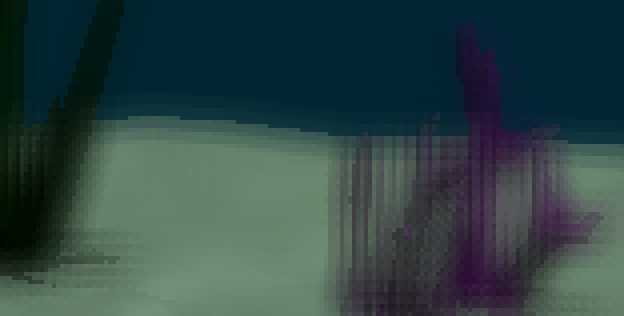
\includegraphics[width=0.6\columnwidth]{imgs/blur_artefacts.png}
	\hspace{1em}
	\caption{Artefacts observed when blurring.}
	\label{fig:blur_artefacts}
\end{figure}


\section{Conclusion}

TODO: Conclude here.

\newpage
\appendix

%% The file named.bst is a bibliography style file for BibTeX 0.99c
\bibliographystyle{named}
\bibliography{ijcai19}

% The reference section will autofill when we add \cite{} in the report.

\end{document}

